\documentclass[lang=cn,11pt,a4paper,cite=authornum]{paper}

\title{Linux开发环境及应用 上机作业二:遍历目录 \\ 实验报告}
\author{毛子恒 \\ 2019211397}
\institute{北京邮电大学\ 计算机学院}

\date{\zhtoday}

\setmonofont{Consolas}

% 本文档命令
\nocite{*}

\begin{document}

\maketitle

\section{实验内容}

编程实现程序\mintinline{text}{list.c},列表普通磁盘文件,包括文件名和文件大小。

\begin{enumerate}
    \item 使用vi编辑文件,熟悉工具vi。
    \item 使用Linux的系统调用和库函数。
    \item 体会Shell文件通配符的处理方式以及命令对选项的处理方式。
\end{enumerate}

\section{实验步骤}

\paragraph{命令行选项获取}

实现一个类似于Linux的\mintinline{text}{getopt}函数\mintinline{text}{getOpt},用于获取命令行选项,该函数依次遍历命令行参数,将获取到的选项返回。全局变量\mintinline{text}{optind}和\mintinline{text}{optarg}分别用于表示遍历到的参数下标以及获取到的参数值。

相比较\mintinline{text}{getopt}函数,我实现的函数稍作简化,无法通过传入参数定制需要解析的命令行选项,但是可以获取到匿名的参数(也就是路径选项)。

\paragraph{打开目录}

\mintinline{text}{match}函数尝试打开传入的路径,并且根据传入的路径是否以'/'结尾做了一些特殊处理,如果指定的路径可以打开,那么调用\mintinline{text}{output}函数输出。

\paragraph{输出}

\mintinline{text}{output}函数判断指定的文件是否满足筛选条件,如果满足则输出,其中还涉及递归输出的过程。

\paragraph{getopt\_long函数的使用}

\mintinline{text}{getopt_long}函数声明如下:

\mintinline{C}{int getopt_long(int argc, char * const argv[], const char *optstring, const struct option *longopts, int *longindex);}

\mintinline{text}{getopt_long}接受长、短的命令行选项,长选项以\mintinline{text}{--}开头。如果程序只接受长选项,那么\mintinline{text}{optstring}应指定为空字符串。如果缩写是唯一的,那么长选项名称可以缩写。长选项可以采用两种形式:\mintinline{text}{--arg=param}或\mintinline{text}{--arg param}。\mintinline{text}{longopts}是结构体\mintinline{text}{option}的数组。

结构体\mintinline{text}{option}的声明如下:

\begin{code}
    \begin{minted}{C}
struct option {
   const char *name;
   int         has_arg;
   int        *flag;
   int         val;
};
\end{minted}
\end{code}

\begin{itemize}
    \item \mintinline{text}{name}:长选项的名字。
    \item \mintinline{text}{has_arg}:0,不需要参数;1,需要参数;2,参数是可选的。
    \item \mintinline{text}{flag}:指定如何为长选项返回结果。如果是NULL,那么函数返回\mintinline{text}{val}(设置为等效的短选项字符),否则返回0。
    \item \mintinline{text}{val}:要返回的值。
\end{itemize}

\mintinline{text}{logopts}数组的最后一个元素必须用零填充。

当一个短选项字符被识别时,\mintinline{text}{getopt_long}也返回选项字符。

\section{代码}

\begin{code}
    \begin{minted}{C}
#include <stdio.h>
#include <string.h>
#include <stdbool.h>
#include <stdlib.h>
#include <ctype.h>
#include <time.h>
#include <unistd.h>
#include <dirent.h>
#include <sys/stat.h>

#ifndef MAXNAMLEN
#define MAXNAMLEN 255
#endif // MAXNAMLEN

char *opt_arg;
int opt_ind = 1;

struct Flags
{
    bool recursive;
    bool all;
    long low;
    long high;
    double modified;
} flags;

char pwd[MAXNAMLEN];

int getOpt(int argc, char *argv[]);

bool match(const char *pattern);

void output(const char *path);

void help_info();

int main(int argc, char *argv[])
{
    int path_args_cnt = 0;
    char **path_args_list = (char **)malloc(argc * sizeof(char *));

    flags.high = flags.modified = 0x7fffffff;
    int ch;
    while ((ch = getOpt(argc, argv)) != -1)
    {
        switch (ch)
        {
        case 0:
            path_args_list[++path_args_cnt] = opt_arg;
            break;
        case 'r':
            flags.recursive = true;
            break;
        case 'a':
            flags.all = true;
            break;
        case 'l':
            flags.low = atoll(opt_arg);
            if (strcmp(opt_arg, "0") && !flags.low)
                help_info();
            break;
        case 'h':
            flags.high = atoll(opt_arg);
            if (strcmp(opt_arg, "0") && !flags.high)
                help_info();
            break;
        case 'm':
            flags.modified = atoll(opt_arg) * 3600 * 24;
            if (strcmp(opt_arg, "0") && !flags.modified)
                help_info();
            break;
        case '?':
            help_info();
            break;
        }
    }

    if (getcwd(pwd, MAXNAMLEN) == NULL)
    {
        fprintf(stderr, "getcwd(): Error.");
        free(path_args_list);
        exit(1);
    }

    if (!path_args_cnt) // no path args, list pwd
    {
        match(pwd);
        free(path_args_list);
        return 0;
    }

    for (int i = 1; i <= path_args_cnt; ++i)
    {
        char *pattern = (char *)malloc((strlen(path_args_list[i]) + MAXNAMLEN + 1) * sizeof(char));
        if (!strlen(path_args_list[i]) || (path_args_list[i][0] == '.' && path_args_list[i][1] != '.'))
        {
            strcpy(pattern, pwd);
            strcpy(pattern + strlen(pwd), path_args_list[i] + 1);
        }
        else if ((path_args_list[i][0] == '.' && path_args_list[i][1] == '.' && path_args_list[i][2] == '/') || strrchr(path_args_list[i], '/') == NULL)
        {
            strcpy(pattern, pwd);
            pattern[strlen(pwd)] = '/';
            strcpy(pattern + strlen(pwd) + 1, path_args_list[i]);
        }
        else
            strcpy(pattern, path_args_list[i]);
        // printf("%s\n", pattern);

        if (!match(pattern))
            fprintf(stderr, "list: cannot access '%s': No such file or directory\n", path_args_list[i]);
        free(pattern);
    }
    free(path_args_list);
    return 0;
}

int getOpt(int argc, char *argv[])
{
    if (opt_ind >= argc)
        return -1;
    if (argv[opt_ind][0] != '-')
    {
        opt_arg = argv[opt_ind];
        opt_ind++;
        return 0;
    }
    if (argv[opt_ind][1] == '-')
    {
        opt_ind++;
        return -1;
    }
    else if (argv[opt_ind][1] == 'r' || argv[opt_ind][1] == 'a')
    {
        opt_arg = NULL;
        char opt = argv[opt_ind][1];
        opt_ind++;
        return opt;
    }
    else if (argv[opt_ind][1] == 'l' || argv[opt_ind][1] == 'h' || argv[opt_ind][1] == 'm')
    {
        if (opt_ind + 1 >= argc)
        {
            opt_arg = NULL;
            return '?';
        }
        else
            opt_arg = argv[opt_ind + 1];
        char opt = argv[opt_ind][1];
        opt_ind += 2;
        return opt;
    }
    else
    {
        opt_ind++;
        return '?';
    }
}

bool match(const char *pattern)
{
    char *last_slash = strrchr(pattern, '/');
    char *last_pattern = (char *)malloc(strlen(pattern) * sizeof(char));
    char *file_name = (char *)malloc(MAXNAMLEN * sizeof(char));
    strncpy(last_pattern, pattern, last_slash - pattern);
    strcpy(file_name, last_slash + 1);

    DIR *dir;
    struct dirent *ent;
    if ((dir = opendir(last_pattern)) == NULL)
    {
        free(last_pattern);
        free(file_name);
        return false;
    }

    if (!strlen(file_name)) // pattern end with '/'
    {
        *last_slash = 0;
        last_slash = strrchr(last_pattern, '/');
        *last_slash = 0;
        strcpy(file_name, last_slash + 1);
        closedir(dir);
        dir = opendir(last_pattern);
    }
    // printf("%s %s\n", last_pattern, file_name);

    while ((ent = readdir(dir)) != NULL)
    {
        if (!strcmp(file_name, ent->d_name))
        {
            output(pattern);
            return true;
        }
    }
    closedir(dir);
    free(last_pattern);
    free(file_name);
    return false;
}

void output(const char *path)
{
    struct stat statbuf;
    stat(path, &statbuf);
    if (S_ISDIR(statbuf.st_mode))
    {
        DIR *dir;
        struct dirent *ent;
        struct stat statbuf;

        if ((dir = opendir(path)) == NULL)
        {
            fprintf(stderr, "Can`t open directory %s\n", path);
            return;
        }

        while ((ent = readdir(dir)) != NULL)
        {
            if (ent->d_name[0] == '.')
                if (!flags.all)
                    continue;
            char *new_path = (char *)malloc((strlen(path) + MAXNAMLEN + 1) * sizeof(char));
            strcpy(new_path, path);
            if (!strcmp(path, "/"))
                strcpy(new_path + 1, ent->d_name);
            else
            {
                strcpy(new_path + strlen(path) + 1, ent->d_name);
                *(new_path + strlen(path)) = '/';
            }
            stat(new_path, &statbuf);
            if (statbuf.st_size >= flags.low && statbuf.st_size <= flags.high && difftime(time(NULL), statbuf.st_mtime) <= flags.modified)
                printf("%10ld %s\n", statbuf.st_size, new_path);
            if (!flags.recursive)
            {
                free(new_path);
                continue;
            }
            if (S_ISDIR(statbuf.st_mode))
            {
                if (!strcmp(ent->d_name, ".") || !strcmp(ent->d_name, ".."))
                    continue;
                output(new_path);
            }
            free(new_path);
        }
    }
    else
    {
        stat(path, &statbuf);
        if (statbuf.st_size >= flags.low && statbuf.st_size <= flags.high && difftime(time(NULL), statbuf.st_mtime) <= flags.modified)
            printf("%10ld %s\n", statbuf.st_size, path);
    }
}

void help_info()
{
    printf("usage: list [-r] [-a] [-l <minimum_size>] [-h <maximum_size>] [-m <modified_days>] [file ...]\n");
    exit(1);
}
\end{minted}
\end{code}

\section{运行结果}

采用如下命令编译:

\begin{code}
    \begin{minted}{shell}
gcc list.c -o list -std=c11 -Wall
\end{minted}
\end{code}

运行结果如\figref{fig:p1}。

\begin{figure}[!htb]
    \centering
    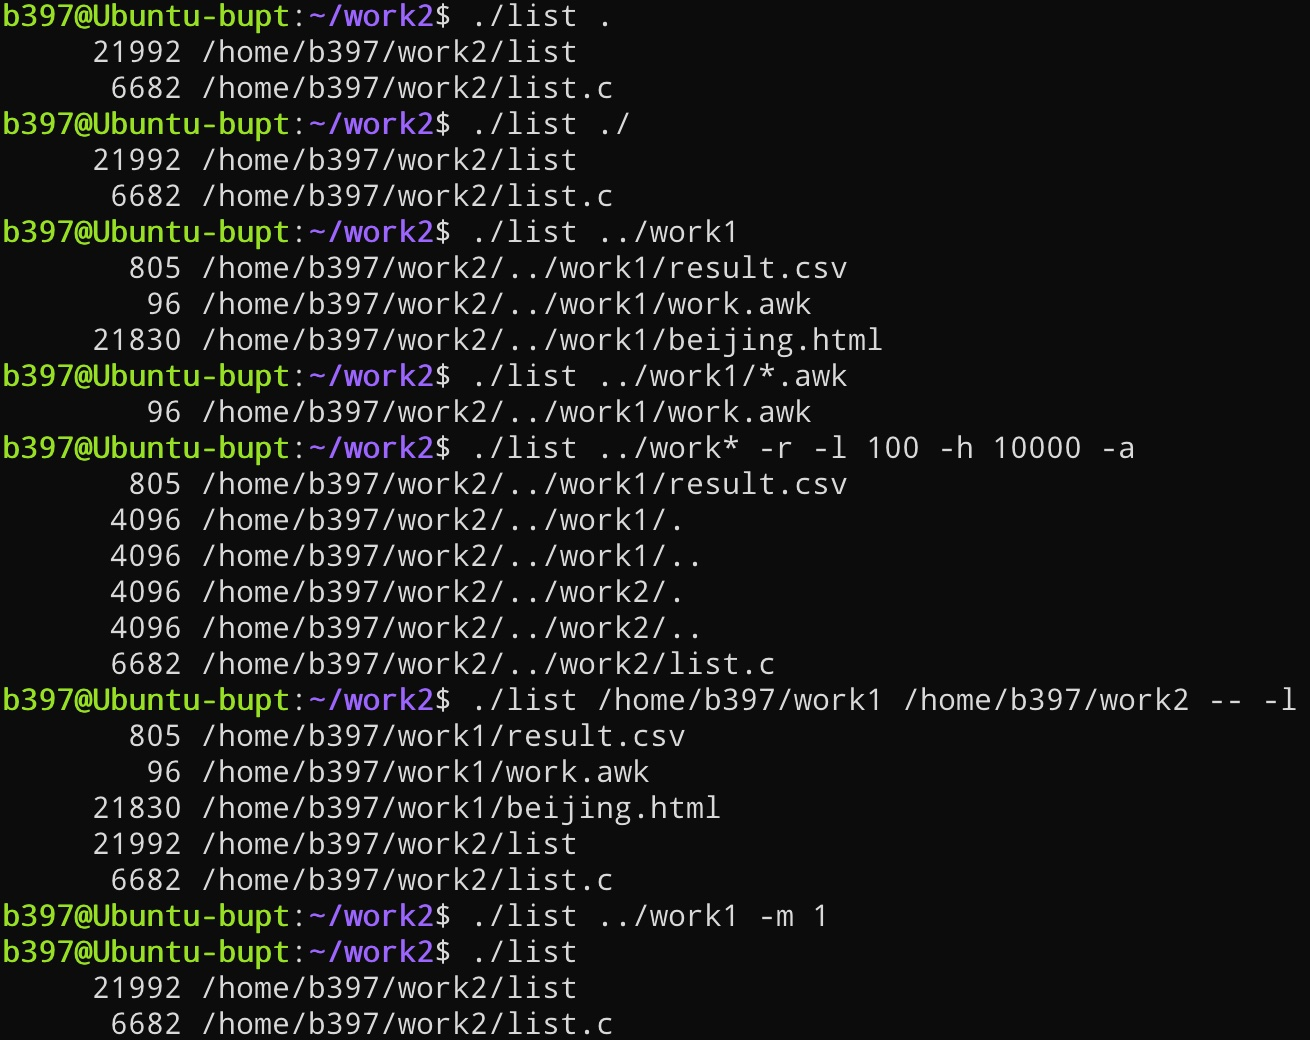
\includegraphics[width=\textwidth]{./images/l2.jpg}
    \caption{运行结果\label{fig:p1}}
\end{figure}

\section{实验总结}

实验期间我观察到Shell会先对通配符进行解析,将其展开为多个参数传递给程序。

本次实验中我应用Linux目录和文件信息访问的库函数,实现了对指定目录的遍历操作,使我对Linux的文件系统理解更加深刻。

\end{document}